\documentclass[12pt,twoside]{article}

\usepackage{amsmath}
\usepackage{amssymb}
\usepackage{amsthm}
\usepackage{array}
\usepackage{amsfonts}
\usepackage[all,cmtip]{xy}%Commutative Diagrams
\usepackage[pdftex]{graphicx}
\usepackage{enumerate}
\usepackage{fancyhdr}
\usepackage{float}
\usepackage{fullpage}
\usepackage[margin=1in]{geometry}
\usepackage{mathrsfs}
\usepackage{sidecap}
\usepackage{tabularx} 
\usepackage{verbatim}
\usepackage{wrapfig}
\usepackage{ctable,booktabs}

\newtheoremstyle{norm}
{3pt}
{3pt}
{}
{}
{\bf}
{:}
{.5em}
{}

\theoremstyle{norm}
\newtheorem{thm}{Theorem}[section]
\newtheorem{lem}[thm]{Lemma}
\newtheorem{df}{Definition}
\newtheorem{rem}{Remark}
\newtheorem{st}{Step}
\newtheorem{pr}[thm]{Proposition}
\newtheorem{cor}[thm]{Corollary}
\newtheorem{conj}[thm]{Conjecture}
\newtheorem{clm}[thm]{Claim}
\newtheorem{exr}[thm]{Exercise}
\newtheorem{ex}[thm]{Example}
\newtheorem{prb}[thm]{Problem}

%Math blackboard, fraktur, and script commonly used letters
\newcommand{\A}[0]{\mathbb{A}}
\newcommand{\C}[0]{\mathbb{C}}
\newcommand{\sC}[0]{\mathcal{C}}
\newcommand{\cE}[0]{\mathscr{E}}
\newcommand{\F}[0]{\mathbb{F}}
\newcommand{\cF}[0]{\mathscr{F}}
\newcommand{\cG}[0]{\mathscr{G}}
\newcommand{\sH}[0]{\mathscr H}
\newcommand{\Hq}[0]{\mathbb{H}}
\newcommand{\N}[0]{\mathbb{N}}
\newcommand{\Pj}[0]{\mathbb{P}}
\newcommand{\sO}[0]{\mathcal{O}}
\newcommand{\cO}[0]{\mathscr{O}}
\newcommand{\Q}[0]{\mathbb{Q}}
\newcommand{\R}[0]{\mathbb{R}}
\newcommand{\Z}[0]{\mathbb{Z}}
%Lowercase
\newcommand{\ma}[0]{\mathfrak{a}}
\newcommand{\mb}[0]{\mathfrak{b}}
\newcommand{\fg}[0]{\mathfrak{g}}
\newcommand{\vi}[0]{\mathbf{i}}
\newcommand{\vj}[0]{\mathbf{j}}
\newcommand{\vk}[0]{\mathbf{k}}
\newcommand{\mm}[0]{\mathfrak{m}}
\newcommand{\mfp}[0]{\mathfrak{p}}
\newcommand{\mq}[0]{\mathfrak{q}}
\newcommand{\mr}[0]{\mathfrak{r}}
%More sequences of letters
\newcommand{\chom}[0]{\mathscr{H}om}
\newcommand{\fq}[0]{\mathbb{F}_q}
\newcommand{\fqt}[0]{\mathbb{F}_q^{\times}}
\newcommand{\sll}[0]{\mathfrak{sl}}
%Shortcuts for symbols
\newcommand{\nin}[0]{\not\in}
\newcommand{\opl}[0]{\oplus}
\newcommand{\ot}[0]{\otimes}
\newcommand{\rc}[1]{\frac{1}{#1}}
\newcommand{\send}[0]{\rightsquigarrow}
\newcommand{\sub}[0]{\subset}
\newcommand{\subeq}[0]{\subseteq}
\newcommand{\supeq}[0]{\supseteq}
\newcommand{\nsubeq}[0]{\not\subseteq}
\newcommand{\nsupeq}[0]{\not\supseteq}
%Shortcuts for greek letters
\newcommand{\al}[0]{\alpha}
\newcommand{\be}[0]{\beta}
\newcommand{\ga}[0]{\gamma}
\newcommand{\Ga}[0]{\Gamma}
\newcommand{\de}[0]{\delta}
\newcommand{\ep}[0]{\varepsilon}
\newcommand{\eph}[0]{\frac{\varepsilon}{2}}
\newcommand{\ept}[0]{\frac{\varepsilon}{3}}
\newcommand{\la}[0]{\lambda}
\newcommand{\La}[0]{\Lambda}
\newcommand{\ph}[0]{\varphi}
\newcommand{\rh}[0]{\rho}
\newcommand{\te}[0]{\theta}
\newcommand{\om}[0]{\omega}
%Brackets
\newcommand{\ab}[1]{\left| {#1} \right|}
\newcommand{\ba}[1]{\left[ {#1} \right]}
\newcommand{\bc}[1]{\left\{ {#1} \right\}}
\newcommand{\pa}[1]{\left( {#1} \right)}
\newcommand{\an}[1]{\langle {#1}\rangle}
\newcommand{\fl}[1]{\left\lfloor {#1}\right\rfloor}
\newcommand{\ce}[1]{\left\lceil {#1}\right\rceil}
%Text
\newcommand{\btih}[1]{\text{ by the induction hypothesis{#1}}}
\newcommand{\bwoc}[0]{by way of contradiction}
\newcommand{\by}[1]{\text{by~(\ref{#1})}}
\newcommand{\ore}[0]{\text{ or }}
%Formatting
\newcommand{\subprob}[1]{\noindent\textbf{#1}\\}
%Functions, etc.
\newcommand{\Ann}{\operatorname{Ann}}
\newcommand{\AP}{\operatorname{AP}}
\newcommand{\Ass}{\operatorname{Ass}}
\newcommand{\chr}{\operatorname{char}}
\newcommand{\cis}{\operatorname{cis}}
\newcommand{\Cl}{\operatorname{Cl}}
\newcommand{\Der}{\operatorname{Der}}
\newcommand{\End}{\operatorname{End}}
\newcommand{\Ext}{\operatorname{Ext}}
\newcommand{\Frac}{\operatorname{Frac}}
\newcommand{\FS}{\operatorname{FS}}
\newcommand{\GL}{\operatorname{GL}}
\newcommand{\Hom}{\operatorname{Hom}}
\newcommand{\Ind}[0]{\text{Ind}}
\newcommand{\im}[0]{\text{im}}
\newcommand{\nil}[0]{\operatorname{nil}}
\newcommand{\Proj}{\operatorname{Proj}}
\newcommand{\Rad}{\operatorname{Rad}}
\newcommand{\Res}[0]{\text{Res}}
\newcommand{\sign}{\operatorname{sign}}
\newcommand{\SL}{\operatorname{SL}}
\newcommand{\Spec}{\operatorname{Spec}}
\newcommand{\Specf}[2]{\Spec\pa{\frac{k[{#1}]}{#2}}}
\newcommand{\spp}{\operatorname{sp}}
\newcommand{\spn}{\operatorname{span}}
\newcommand{\Supp}{\operatorname{Supp}}
\newcommand{\Tor}{\operatorname{Tor}}
\newcommand{\tr}[0]{\text{trace}}
%Commutative diagram shortcuts
\newcommand{\fiber}[3]{\xymatrix{#1\times_{#3} #2}\ar[r]\ar[d] #1\ar[d] \\ #2 \ar[r] & #3}
%Other
\newcommand{\op}{^{\text{op}}}
\newcommand{\fp}[1]{^{\underline{#1}}}
\newcommand{\rp}[1]{^{\overline{#1}}}
\newcommand{\rd}[0]{_{\text{red}}}
\newcommand{\pre}[0]{^{\text{pre}}}
\newcommand{\pf}[2]{\pa{\frac{#1}{#2}}}
\newcommand{\pd}[2]{\frac{\partial #1}{\partial #2}}
%Matrices
\newcommand{\coltwo}[2]{
\left[
\begin{array} {c}
{#1}\\
{#2} 
\end{array}
\right]}
\newcommand{\matt}[4]{
\left[
\begin{array} {cc}
{#1}&{#2}\\
{#3}&{#4}
\end{array}
\right]}
\newcommand{\colthree}[3]{
\left[
\begin{array} {c}
{#1}\\
{#2}\\
{#3}
\end{array}
\right]}
%Page breaks in equations
\allowdisplaybreaks[1]

% Do not change any of this
\pagestyle{fancy}
\lhead{\textit{OMC 2010}}

\chead{The Beauty of Mathematics}

%%%%%%%%%%
% LECTURE NUMBER
%%%%%%%%%%
\rhead{\textit{Lecture 1}}

\headheight 0cm
\setlength{\headsep}{18pt}
\setlength{\headheight}{15.2pt}

%%%%%%%%%%
% CONTENT
%
% Here is where you place the problems and any other content. If you are making a problem set, use the \item command to create a new problem. 
%
%%%%%%%%%%
\begin{document}
\title{Lecture $1$ --- The Beauty of Mathematics}% !! Remember to change the lecture number
\author{Holden Lee}
\date{December 4, 2010}% !! Remember to change the date
\maketitle
\thispagestyle{empty}
\section{Playing with Numbers}
%One of the most beautiful things about 
Mathematics makes it possible to embark on a journey of discovery armed with a brain, pencil, and paper. You don't need to be at the frontiers of mathematical research, nor learn years of graduate school math to find this pleasure for yourself. All it takes is some curiosity about why things are true, and a willingness to try something without knowing in advance whether it will work.

To illustrate this, we will start with a simple question about decimal expansions, and show how it can lead naturally to some interesting math, motivate the foundations of number theory, and give even more unanswered questions. To make this more hands-on, exercises are included throughout; please give them some thought!

When I was a kid, I liked to compute the decimal expansions of fractions:
\begin{align*}
\rc{2}&=.5\\
\rc{3}&=.\overline{3}\\
\rc{4}&=.25\\
\rc{5}&=.2\\
\rc{6}&=.1\overline{6}\\
\rc{7}&=.\overline{142857}\\
\rc{8}&=.125\\
\rc{9}&=.\overline{1}\\
\rc{10}&=.1\\
\rc{11}&=.\overline{09}\\
\rc{12}&=.08\overline{3}\\
\rc{13}&=.\overline{076923}\\
\rc{17}&=.\overline{0588235294117647}\\
\rc{19}&=.\overline{052631578947368421}
\end{align*}
We could go on and on... but let's take a look at what we have so far. One natural question we could ask is: when is $\rc{n}$ a terminating decimal, and when it is repeating? If it is repeating, what is its period?

Actually, before we answer these questions, we should ask ourselves why it is that all these decimals either repeat or terminate, in the first place. To answer this question, we can think about how decimal expansions are computed. Consider the case of $\rc 7$.
\[
\begin{tabular}{cccccccc}
 & 0. & 1 & 4 & 2 & 8 & 5 & 7\tabularnewline
\cline{2-8} 
\multicolumn{1}{c|}{7} & \textbf{1}. & 0 & 0 & 0 & 0 & 0 & 0\tabularnewline
 & $-$ & 7 &  &  &  &  & \tabularnewline
\cline{2-3} 
 &  & \textbf{3} & 0 &  &  &  & \tabularnewline
 & $-$ & 2 & 8 &  &  &  & \tabularnewline
\cline{3-4} 
 &  &  & \textbf{2} & 0 &  &  & \tabularnewline
 &  & $-$ & 1 & 4 &  &  & \tabularnewline
\cline{4-5} 
 &  &  &  & \textbf{6} & 0 &  & \tabularnewline
 &  &  & $-$ & 5 & 6 &  & \tabularnewline
\cline{5-6} 
 &  &  &  &  & \textbf{4} & 0 & \tabularnewline
 &  &  &  & $-$ & 3 & 5 & \tabularnewline
\cline{6-7} 
 &  &  &  &  &  & \textbf{5} & 0\tabularnewline
 &  &  &  &  & $-$ & 4 & 9\tabularnewline
\cline{7-8} 
 &  &  &  &  &  &  & \textbf{1}\tabularnewline
\end{tabular}\]
We start out with 1, add a 0 to get 10, find the greatest multiple of 7 that goes into 10, subtract, then do the same thing with the remainder 3. 
We carry down a 0 to get 30, find the greatest multiple of 7 that goes into 30, 
and subtract to get a new remainder 2. The key point is that all the remainders are between 0 and 6 (in general, between 0 and $n-1$), so at some stage one of them must repeat (Pigeonhole Principle!). 
If at step $t_1$ and step $t_2>t_1$, the remainders are the same, then the steps carried out after step $t_2$ will be exactly the same as the steps 
carried out after $t_1$, since at each stage we only care about the last remainder we computed. If we hit 0 at some stage, then we are done---the decimal terminates. 
Else we will be caught in some loop that has length at most $n-1$. This reasoning actually works for all fractions (though we might have some ``random" numbers at the beginning, before we start carrying 0's). Thus we have proved the following.
\begin{thm}\label{ratexp}
Every rational number has a terminating or periodic decimal expansion. Moreover, if $\frac{m}{n}$ has a periodic expansion, then its period is at most $n-1$.
\end{thm}
\begin{exr}
Which values of $n$ cause $\rc{n}$ to terminate? For these values of $n$, how long is the decimal expansion?
\end{exr}
%\begin{exr}
%If the maximum $n-1$ is attained, what can you conclude about $n$?
%\end{exr}
Now let's investigate some of the questions we posed before. We print the same fractions again, this time including the periods:
\begin{align*}
&&\text{Period}\\
\rc{2}&=.5&\text{Terminating}\\
\rc{3}&=.\overline{3}&1\\
\rc{4}&=.25&\text{Terminating}\\
\rc{5}&=.2&\text{Terminating}\\
\rc{6}&=.1\overline{6}&1\\
\rc{7}&=.\overline{142857}&6\\
\rc{8}&=.125&\text{Terminating}\\
\rc{9}&=.\overline{1}&1\\
\rc{10}&=.1&\text{Terminating}\\
\rc{11}&=.\overline{09}&2\\
\rc{12}&=.08\overline{3}&1\\
\rc{13}&=.\overline{076923}&6\\
\rc{17}&=.\overline{0588235294117647}&16\\
\rc{19}&=.\overline{052631578947368421}&18
\end{align*}
The more interesting expansions seem to happen when the denominator is prime. We make the following observations.
\begin{enumerate}
\item The expansion of $\rc p$ seems to always be periodic from the beginning (as opposed to something like $\rc{6}=.1\overline 6$).
\item The expansion for $\rc 7$ has 6 digits, the expansion for $\rc{17}$ has 16 digits, and the expansion for $\rc{19}$ has 18 digits; they achieve the ``maximum" possible cycle. Moreover, the maximum period as given in Theorem~\ref{ratexp} is only attained when the denominator is prime.
\item Not all primes have the maximum possible cycle length; for example, $\rc{13}$ has period 6. However, $6$ is a factor of $13-1$. It seems that the period for $\rc{p}$ $p\neq 2,5$ is a factor of $p-1$.
\end{enumerate}
%One especially intriguing fact is that t Why would this be the case? What do these numbers have in common? They are all primes. 
From now on we'll concentrate on $\rc p$ when $p$ is prime, and not equal to 2 or 5. We've calculated $\rc 7$, so why not calculate $\frac{n}{7}$ as well, for other values of $n$:
\begin{align*}
\frac{1}{7}&=.\overline{142857}\\
\frac{2}{7}&=.\overline{285714}\\
\frac{3}{7}&=.\overline{428571}\\
\frac{4}{7}&=.\overline{571428}\\
\frac{5}{7}&=.\overline{714285}\\
\frac{6}{7}&=.\overline{857142}
\end{align*}
Notice how the numbers in the repeating part cycle. Does this work for other primes $p$ for which $\rc{p}$ has period $p-1$? Let's try $\frac{1}{17}$:
\begin{align*}
\frac{1}{17}&=.\overline{0588235294117647}\\
\frac{2}{17}&=.\overline{1176470588235294}\\
\frac{3}{17}&=.\overline{1764705882352941}\\
\frac{4}{17}&=.\overline{2352941176470588}\\
\ldots
\end{align*}
Yes it does! (You can compute the others if you'd like.) From these examples we make the following conjecture.
\begin{conj}
If $\rc{p}$ has $p-1$ digits in its repeating part, then $p$ is prime; moreover, the expansions of $\frac{n}{p}$ for $1\leq n<p$ have the same repeating part as $\rc{p}$ but shifted.
\end{conj}
%Let's call these prime numbers {\it special}. 
Shifting periods seems to suggest multiplying by 10, so we calculate
\begin{align*}
\frac{1}{7}&=\;\;\;\;\;\;\;\;\;\;.\mathbf{142857}142857\ldots\\
\frac{10}{7}=1\frac{3}{7}&=\;\;\;\;\;\;\;\;1.\mathbf{428571}42857\ldots\\
\frac{100}{7}=14\frac{2}{7}&=\;\;\;\;\;\;14.\mathbf{285714}2857\ldots\\
\frac{1000}{7}=142\frac{6}{7}&=\;\;\;\;142.\mathbf{857142}857\ldots\\
\frac{10000}{7}=1428\frac{4}{7}&=\;\;1428.\mathbf{571428}57\ldots\\
\frac{100000}{7}=14285\frac{5}{7}&=14285.\mathbf{714285}7\ldots
\end{align*}
On the left, we multiply the fractions, and on the right we multiply the decimals. Now the fractional parts on the left correspond to the expansions after the decimal points on the right. Notice that the fractional parts on the left cycle through all the fractions $\frac n7$ for $1\leq n<7$. So the reason that the repeating parts cycle is because when we keep  multiplying $\frac 17$ by 10, the fractional parts cycle through {\it all} of the fractions $\frac n7$. In general, if $\rc p$ has period $p-1$, then we get $p-1$ different decimals on the right, which must correspond to different fractions on the left---so all the fractions $\frac np$ have repeating parts that are shifted, as we wanted.

Note that the sequence $1,3,2,6,4,5$ of numerators above is exactly the same as the sequence of remainders upon long division. Can you express the proof of Theorem~\ref{ratexp} using the idea above?

Rather than having to say ``fractional part" all the time, we'll introduce some notation. What we really care about are the numerators of the fractions on the left, which are the remainders when $10^n$ are divided by $7$.
\begin{df}
We denote by $n\pmod{m}$ the remainder of $n$ when divided by $m$. We say that $a\equiv b\pmod{m}$ when $a$ and $b$ leave the same remainder when divided by $m$.
\end{df}
%Rephrasing our observation above
In this new language, a prime $p$ gives the maximal period if and only if $10^n\pmod{p}$ cycles through all the nonzero remainders modulo $p$. This means that $1, 10, \ldots, 10^{p-2}$ are all distinct, and $p-1$ is the smallest value of $n$ so that $10^n\equiv 1\pmod{p}$. %Note that the sequence of remainders (1, 3, 2, 6, 4, 5) is exactly the sequence we got when we carried out long division---think this through! Hence if the length of the repeating part is $p-1$, then repeatedly multiplying $\rc p$ by 10 gives the expansions of all the $\frac{n}{p}$; this shows the second part of our conjecture. Incidentally, all this is related to an important idea in number theory:
\begin{df}
Let $p$ be a prime. A number $d$ is a primitive root modulo $p$ if $p-1$ is the smallest value of $n$ for which $d^{n}\equiv 1\pmod{p}$.
\end{df}

With our new way of thinking, we can now rephrase our questions.
\begin{enumerate}
\item
Why is the expansion of $\rc p$ periodic from the beginning? %This happened with all the primes we looked at, but it's not immediately obvious. 
This is equivalent to saying, if the first repeat in the sequence $1, 10, 10^2,\ldots $ happens at $10^n$, then $10^n\equiv 1\pmod{p}$.
\item 
What is the period of $\rc p$? Assuming the result above, this is equivalent to asking: What is the least number $n$ such that $10^{n}\equiv 1\pmod{p}$? Such $n$ is called the \textbf{order} of $10$ modulo $p$. We'd like to show that the order divides $p-1$.
\end{enumerate}
Let's tackle the first question.
If the first repeat happened at $10^n$, and $10^n\equiv 10^m\pmod{p}$, with $m<n$ and $m\neq 0$, then cancelling a factor 10 on both sides we get that $10^{n-1}\equiv 10^{m-1}\pmod{p}$, which would contradict the minimality of $n$. But wait---we don't know that we can divide by 10 modulo $p$. 
However, all is not lost. The above argument suggests that we show $10a\equiv 10b\pmod{p}$ implies $a\equiv b\pmod{p}$. The first congruence says that $p$ divides $10(a-b)$. But $p$ doesn't divide $10$ so it divides $a-b$, i.e. the second congruence holds, as needed\footnote{If $p$ has no proper divisors (is ``prime"), and $p$ divides $ab$, then either $p$ divides $a$ or $p$ divides $b$. This is in fact not obvious but we'll take it for granted here.}. In fact, this argument generalizes to prove the following.
\begin{thm}\label{canc}
If $m$ is relatively prime to $n$, and $ma\equiv mb\pmod{n}$, then $a\equiv b\pmod{n}$.
\end{thm}

Now let's tackle the second question. As an example we look at $\rc{13}$. We could use the same idea of multiplying fractions by 10, but this time we need {\it two} fractions to generate everything:
\begin{align*}
\frac{1}{13}&=\;\;\;\;\;\;\;\;.\mathbf{076923}076923&
\frac{2}{13}&=\;\;\;\;\;\;\;\;\;\;.\mathbf{153846}153846\\
\frac{10}{13}&=\;\;\;\;\;\;0.\mathbf{769230}76923&
\frac{20}{13}=1\frac{7}{13}&=\;\;\;\;\;\;\;\;1.\mathbf{538461}53846\\
\frac{100}{13}=7\frac{9}{13}&=\;\;\;\;\;\; 7.\mathbf{692307}6923&
\frac{200}{13}=15\frac{5}{13}&=\;\;\;\;\;\;15.\mathbf{384615}3846\\
\frac{1000}{13}=76\frac{12}{13}&=\;\;\;\; 76.\mathbf{923076}923&
\frac{2000}{13}=153\frac{11}{13}&=\;\;\;\;153.\mathbf{846153}846\\
\frac{10000}{13}=769\frac{3}{13}&=\;\; 769.\mathbf{230769}23&
\frac{20000}{13}=1538\frac{6}{13}&=\;\;1538.\mathbf{461538}46\\
\frac{100000}{13}=7692\frac{4}{13}&= 7692.\mathbf{307692}3&
\frac{200000}{13}=15384\frac{8}{13}&=15384.\mathbf{615384}6%\\
%\frac{1000000}{13}=76923\frac{1}{13}&=\;\; 769.\mathbf{230769}23&
%\frac{20000}{13}=1538\frac{6}{13}&=1538.\mathbf{461538}46\\
%
\end{align*}
In general, we take $\frac{1}{p}$, keep multiplying by 10 to get all cyclic permutations of the repeated part, then take a fraction not on our list, and repeat the same argument. So the reason that the period divides $p-1$ is that the fractions $\frac{n}p$ can be grouped into several cycles, each of which has the same period.

%To make this more rigorous, 
We need to establish that each cycle does indeed have the same length. But this follows since we can get to any other cycle by multiplying $\rc p$ by an appropriate factor---above we multiplied the fractions on the left by 2 to get the fractions on the right. Distinct fractional parts will stay distinct, because of Theorem~\ref{canc}.

We could of course state the above argument using the language of modular arithmetic.
\begin{exr}
Do so.
\end{exr}
This verifies our three observations. However, there are a lot more questions that come up, which are left to the reader.
\begin{exr}
What are the possible periods of $\frac{m}{n}$ if $n$ is composite? Are the periods necessarily the same as $m$ varies between 1 and $n-1$? If $a,b$ are relatively prime and you know the period of $\rc a,\rc b$, what is the period of $\rc{ab}$?
\end{exr}
\begin{exr}
Suppose we use a base other than 10. How do our results generalize?
\end{exr}
\begin{exr}
For a prime $p$, $\rc{p}$ in base 10 may not have period $p-1$. But does there exist a base $b$ such that $\rc{p}$ in base $b$ has period $p-1$? Note that if $a\equiv b\pmod{p}$ then $\rc{p}$ has the same period in bases $a$ and $b$. What is the distribution of periods of $\rc{p}$ when $b$ ranges through all nonzero residues modulo $p$?
\end{exr}
\begin{exr}
We've shown that any rational number is a repeating or terminating decimal. Show that any repeating or terminating decimal can be written is in fact rational, and give a way to find this fraction. 
\end{exr}
\begin{exr}
Note that
\[\frac{1}{98}=.0\overline{102040816326530612244897959183673469387755}.\]
Can you explain this? What other fractions give a similar pattern?

[AIME-style problem] Let the 119th, 120th, and 121st digits to the right of the decimal point in $\frac{1}{9999999993}$ be $x,y,z$, respectively. Given that $1.3\times 10^{10}<7^{12}<1.39\times 10^{10}$, find $100x+10y+z$.
\end{exr}
\begin{prb}(Unsolved)
Do there exist infinitely many primes $p$ such that the expansion of $\rc p$ has length $p-1$? If so what proportion of primes (asymptotically) satisfy this? (In other words, are there infinitely many $p$ such that 10 is a primitive root modulo $p$?)
\end{prb}
\section{Counting Change}
%The language of mathematics can give surprising ways to solve p
We'll take a new look at the old problem:
\[
\text{
How many ways are there to give change for \$1?
}
\]
Let's try and find the number of ways $a_c$ to make change for $c$ cents. For simplicity, we'll just count the number of ways to do so with pennies, nickels, dimes, quaters, and half-dollars. Let's represent these coins by the symbols $(1),(5),(10), (25)$, and $(50)$ respectively. We'll let something like
\[
(10)(5)(1)(1)
\]
mean ``1 dime, 1 nickel, and 2 pennies." (The order doesn't matter.) We could sum up all possible combinations of coins as follows:
\begin{equation}\label{sumcoins}
S=1+(1)+(5)+(10)+(25)+(50)+(1)(1)+(5)(1)+(10)(1)+\cdots.
\end{equation}
(Here 1 represents ``0 coins.") 
To find how many ways to get coins adding up to $c$ cents, we could just count how many terms above have their coins summing up to $c$ cents. This doesn't seem very helpful, until we make two key observations:
\begin{enumerate}
\item If we replace $(1)$ by $x$, $(5)$ by $x^5$, $(10)$ by $x^{10}$, $(25)$ by $x^{25}$ and $(50)$ by $x^{50}$, then all terms totalling to $c$ cents collapse to $x^c$. Hence the coefficient of $x^c$ will just be the total number of ways to give change for $c$ cents.
\item We can factor equation~(\ref{sumcoins})! Indeed, specifying a collection of coins is the same thing as specifying some number of pennies, some number of nickels, some number of dimes, some number of quarters, and some number of half-dollars, so
\begin{equation}\label{factorcoin}
\begin{split}
S=&(1+(1)+(1)^2+\cdots)(1+(5)+(5)^2+\cdots)(1+(10)+(10)^2+\cdots)\\
&(1+(25)+(25)^2+\cdots)(1+(50)+(50)^2+\cdots).
\end{split}
\end{equation}
\end{enumerate}
Making the substitution in item 1 into equation~(\ref{factorcoin}), the above says that 
$a_c$ is the coefficient of $x^c$ in
\[
F(x)=(1+x+x^2+\cdots)(1+x^5+x^{10}+\cdots)(1+x^{10}+x^{20}+\cdots)
(1+x^{25}+x^{50}+\cdots)(1+x^{50}+x^{100}+\cdots).
\]
This is called the {\textbf generating function} for our sequence $a_c$. 
We've reduced a combinatorics problem to a purely algebraic one! So now we have all the algebraic and analytic tools at our disposal. We can use the formula for geometric series to get
\begin{align*}
F(x)&=\rc{1-x}\rc{1-x^5}\rc{1-x^{10}}\rc{1-x^{25}}\rc{1-x^{50}}\\
&=\frac{1+x+x^2+x^3+x^4}{1-x^5}\rc{1-x^5}\rc{1-x^{10}}\rc{1-x^{25}}\rc{1-x^{50}}\\
&=(1+x+x^2+x^3+x^4)\rc{(1-y)^2}\rc{1-y^2}\rc{1-y^5}\rc{1-y^{10}}
\end{align*}
where we set $y=x^5$. (This way we have smaller powers to work with. Note that the number of ways to make change for $5k$ cents is the same as the number of ways to make change for $5k+1,5k+2,5k+3,5k+4$ cents; this is reflected above as the coefficients of $x^{5k+c}$ for $0\leq c\leq 4$ will be the same.) We have
\begin{equation}\label{bigformula}
\rc{(1-y)^2}\rc{1-y^2}\rc{1-y^5}\rc{1-y^{10}}
=\frac{(1+y+y^2+\cdots +y^9)^2(1+y^2+\cdots +y^8)(1+y^5)}{(1-y^{10})^5}
\end{equation}
We get a common denominator so we can use the binomial formula
\[
(1+t)^n=\sum_{k=0}^{\infty} \binom{k}{n}t^n.
\]
which in our case reads\footnote{Here $\binom{m}{n}$ is defined as $\frac{m(m-1)\cdots (m-n+1)}{n!}$. For now you can just accept the binomial formula from calculus, since it's not the main point here.} (since $\binom{-k}{n}=(-1)^n\binom{n+k-1}{n}=(-1)^n\binom{n+k-1}{k-1}$)
\begin{equation}\label{binome}
(1-y^{10})^{-5}=\sum_{n=0}^{\infty} \binom{n+4}{4}y^{10n}.
\end{equation}
Hence if we let $g(y)=b_0+b_1y+b_2y^2+\cdots $ denote the numerator to equation~(\ref{bigformula}), we get that the coefficient of $y^{10q+r}, 0\leq r<10$ in~(\ref{bigformula}) is
\[
d_{10q+r}=
\binom{q+4}{4}b_r + \binom{q+3}{4}b_{r+10} + \binom{q+2}{4}b_{r+20} + \binom{q+1}{4}b_{r+30}.
\]
The first term is the product of the coefficient of $y^{10q}$ from equation~(\ref{binome}) and the coefficient of $y^r$ from $g(y)$, the second term is the product of the coefficient of $y^{10(q-1)}$ from~(\ref{binome}) and the coefficient of $y^{10+r}$ from $g(y)$, and so forth. This gives a closed formula for $a_c$:
\begin{equation}\label{coinfinal}
a_{5(10q+r)+s} = \binom{q+4}{4}b_r + \binom{q+3}{4}b_{r+10} + \binom{q+2}{4}b_{r+20} + \binom{q+1}{4}b_{r+30}.
\end{equation}
where $0\leq s\leq 4$. 
All that remains is to actually expand $g(y)$. We'll just work out the formula for multiples of 50 cents. If we expand $g(y)$, then we find that $b_0=1, b_{10}=45,b_{20}=52, b_{30}=2$, so putting $r=0$, $s=0$,
\[
a_{50q}=\binom{q+4}{4} + 45\binom{q+3}{4} + 52\binom{q+2}{4} + 2\binom{q+1}{4}.
\]
In particular, putting $q=2$ gives
\[a_{100}=\binom 64+45\binom 54+52\binom 44=292.\]
Thus the number of ways to get change for \$1 is \textbf{293} (if we include the dollar bill as well). For the curious, the expansion of $g(y)$ is
\begin{align*}
&1+2y+4y^2+6y^3+9y^4+13y^5+18y^6+24y^7+31y^8+39y^9\\
+&45y^{10}+52y^{11}+57y^{12}+63y^{13}+67y^{14}+69y^{15}+69y^{16} +67y^{17} +63y^{18} +57y^{19}\\
+&52y^{20}+45y^{21}+39y^{22}+31y^{23}+24y^{24}+18y^{25}+13y^{26}+9y^{27}+6y^{28}+4y^{29}+2y^{30}+y^{31}
\end{align*}
\begin{exr}
Can you give a combinatorial interpretation of~(\ref{coinfinal})?
\end{exr}
\begin{exr}
Let $a_n$ denote the number of ways to tile a $2\times n$ board with dominoes. Find a generating function for $a_n$. (Hint: The order of the dominoes matters in this case!)

(Harder) Can you generalize to a $3\times n$ board?
\end{exr}
\section{Fun with Cannibals}

\footnote{This section is based off a lecture by Brian Basham at AwesomeMath Summer Program 2010.}
Suppose that, while vacationing on a desert island, you and two friends are captured by cannibals. The cannibals decide to play the following game. They place a black or white hat on each person's head, independently with probability $\rc 2$, so that no one can see his or her own hat, but can see the hats of everyone else. At the count of three, each person may either guess the color of his hat, or stay silent.
\begin{itemize}
\item
If at least one person guesses, and if everyone guesses correctly, then you are all released.
\item 
If anyone guesses wrong, or no one ventures to guess, then everyone is eaten by cannibals.
\end{itemize}
The cannibals tell you the rules beforehand, and allow you to discuss your plans. What is your optimal strategy?

Note that a strategy for this game tells each person what to do under all of the 4 possible color combinations of the other people's hats.

\begin{exr}
At first glance, it might seem like there there is no way to have a better chance than $\rc 2$ of being released. We might argue like this: In any situation, someone has to make a guess, if you are to win. There are two possible colors for that person's hat color, and both are equally likely. Hence the probability of guessing correctly is $\rc 2$, so the overall probability of escaping alive is at most $\rc 2$. What is wrong with this argument? Try to answer this (and maybe think about the problem a bit!) before reading the answer on the next page.
\end{exr}
\pagebreak
The best strategy gives a $\frac 34$ chance of success. The strategy is as follows: anyone who sees two hats of different colors stays silent, while anyone who sees two hats of the same color guesses the other color. Then when there are two different hat colors, exactly one person will guess, and he will guess correctly, while if all hats are the same color, then everyone will guess incorrectly. These cases cover 6 and 2 out of the 8 total possibilities, respectively, giving the probability of $\frac 34$.

\begin{figure}[h!]
\centering
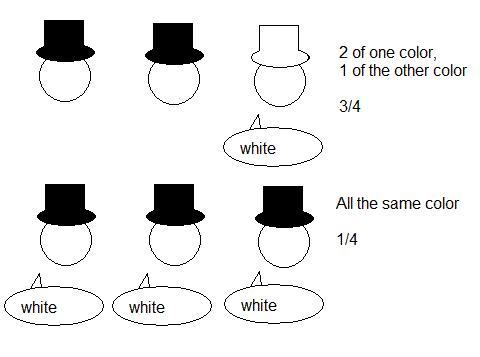
\includegraphics{hats}
\end{figure}

It is true that if we add up the total number of correct guesses in all 8 possible cases, it will equal the total number of incorrect guesses. However, note that all the instances of incorrect guesses are concentrated in the ``bad case" where everyone wore the same color hat.

Now we can ask the same question with different numbers of people. If we increase the number of people, do the odds of success increase? In fact, we will show even more:
\begin{thm}
As the number of people tend to infinity, the probability of success (using the best strategy) {\it tends to 1}.
\end{thm}
First, let's use the counting argument suggested above to find an upper bound for the probability of success. Fix a strategy and suppose there are $n$ people; then there are $2^n$ equally probable possibilities for their hat colors. Suppose in $w$ of them, their strategy will allow them to go free. 
In each such case, someone guessed correctly; thus there must be a corresponding case, where the color of that person's hat is switched, in which that person guesses wrong. The total number of incorrect guesses summed over all cases is at least $w$. In each case, there can be at most $n$ wrong guesses (since there are $n$ people); therefore at least $\frac wn$ of the cases contain a wrong guess. These cases cannot overlap with the $w$ cases where the prisoners are allowed free, so
\begin{align}
\nonumber \frac wn+w&\leq 2^n\\
w&\leq \frac{n}{n+1}2^n\label{hateq}
\end{align}
Thus the probability of success is at most $\frac{n}{n+1}$. This is exciting, because it approaches 1 as $n$ goes to infinity; however we have to see if it's actually attainable.

Note this agrees with our answer for $n=3$. In general the optimal bound cannot be attained, because $2^n$ is not necessarily a multiple of $n+1$. It may be attainable when $n$ is in the form $2^k-1$, so let's focus on this case. Our solution will have to depend on the fact that $n$ is in this form; one way to use this fact is that it allows us to label the people from $1$ to $2^k-1$ in binary, i.e. each person can be labeled with a sequence of $k$ 0's and 1's, which is not all 0's. For example, with 7 people we label them by 3-digit sequences: (we omit the 0's)
\[
\begin{tabular}{c|c|c|c|c|c|c|c}
 & 1 & 2 & 3 & 4 & 5 & 6 & 7\tabularnewline
\hline
$2^{0}$ & 1 &  & 1 &  & 1 &  & 1\tabularnewline
$2^{1}$ &  & 1 & 1 &  &  & 1 & 1\tabularnewline
$2^{2}$ &  &  &  & 1 & 1 & 1 & 1\tabularnewline
\end{tabular}
\]
In order to attain our bound, we need to choose $\frac{1}{n+1}$ of the $2^n$ cases to be ``bad" cases, and have people guess that they are not in a bad case. This is like the $n=3$ case, where we designated all white or all black hats as the bad cases, and if from person $P$'s point of view he could be in a bad case, $P$ guesses that his hat color is different from the bad case; this is good since there are few bad cases. 

One way to visualize this is as follows: we associate each sequence of $n$ hats with a sequence of $n$ 0's and 1's, with white being 0 and black being 1. This matches the $2^n$  possibilities with the points of a hypercube in $n$ dimensions. Two cases which differ by one hat color correspond to adjacent points.
Each point has $n$ incident edges, leading to points differing in one of $n$ possible coordinates. 
Each edge corresponds to $n-1$ fixed hat colors and one unknown hat color; think of the $n$ edges from the vertex as describing what the $n$ people see---each sees the other $n-1$ color but is unsure of his own.
We call a point good if it corresponds to a winning case under the strategy, and bad (or special) otherwise. Rephrasing in our new language,
\begin{enumerate}
\item
A person's guess given the other people's hat colors corresponds to a fixed direction for the edge corresponding to what he sees, the arrow pointing towards the guess.
\item
If at every vertex there is at least 1 directed edge incident to it, and all those edges point inwards, then it is a good point. The $n$ edges around a point represent what the $n$ people see in the corresponding case, and the inward edge corresponds to someone making the correct guess.
\item
For equality to be attained in~(\ref{hateq}), all bad vertices must have all incident edges pointing away from it.
\end{enumerate}
For $n=3$, the cube looks like the above.
\begin{figure}[h!]
\centering
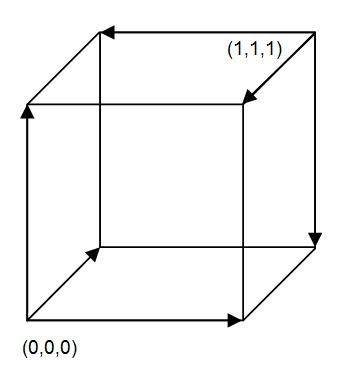
\includegraphics[scale=0.5]{hypercube}
\end{figure}

In the general case, we would like to choose $\rc{n+1}=\rc{2^k}$ points from the $2^n$ points to designate as ``special" points, such that every non-special point is adjacent to exactly one special point. Then we have people guess that are not at a special point, like before. For a point in the hypercube, write its coordinates in the table, mark all the columns where 1 appears, and sum across the rows. 
We say the point is special if all the sums are even---observe that this happens $\rc{2^k}$ of the time as we would like. Now every point is adjacent to exactly one special point, because there's exactly one nonzero number in binary we could add to it digit-wise to get all evens in the last row; in the example below it is 5 (101), so the adjacent point is $(1,1,0,0,1,1,0)$.
\[
\begin{tabular}{c|c|c|c|c|c|c|c|c}
 & 1 & 2 & 3 & 4 & 5 & 6 & 7 & Total marked\tabularnewline
\hline
$2^{0}$ & \textbf{1} &  & 1 &  & 1 &  & 1 & 1\tabularnewline
$2^{1}$ &  & \textbf{1} & 1 &  &  & \textbf{1} & 1 & 2\tabularnewline
$2^{2}$ &  &  &  & 1 & 1 & \textbf{1} & 1 & 1\tabularnewline
point & 1 & 1 & 0 & 0 & 0 & 1 & 0 & \tabularnewline
\end{tabular}
\]
In this case, person 5 would guess white, and be correct.

Thus, summarizing, everyone is assigned a sequence of 0's and 1's; in the game each person sums up digit-wise the sequences of all people who are wearing black hats, then determines if either including or excluding his own sequence would cause all the entries to be even. If so, then he %is the ``special" person, and he 
guesses the hat color that would cause the sum to not have all entries even. Since it is unlikely that the digit-wise sum of the people wearing black hats will be all even, it is likely that he will guess correctly. This is the optimal strategy for $n=2^k-1$, so as $n\to \infty$, we can make the probability of success not only greater than $\rc2$, but in fact as close to 1 as we want! (If $n$ is not in the form $2^k-1$, we can carry out this strategy with just $2^k-1<n$ of the people.)

Though this problem is ``just for fun," it actually touches on an interesting application of mathematics to computer science: When data is transmitted  errors accumulate due to various reasons, and the computer or device receiving the data must be able to correct them. So instead of having all strings of 0's and 1's represent valid data, only certain combinations do; then when a string is not valid, we know that an error has occurred and we guess that it is supposed to be the valid sequence closest to the received sequence (differing in the least number of places). In our above choice of ``special" points, we made sure that each other point was adjacent to exactly one special point. This way, if there's an error in a single bit then we can recover the original data, just like we found the unique adjacent special point. Without such error correction, data would get garbled so easily that our familiar electronics would no longer work.

Here's some related puzzles to think about.
\begin{exr}(based off UM 2009)
Again, the cannibals place a black or white hat on everyone's head. Suppose that everyone is required to guess their own hat color, and everyone who guesses correctly survives, while everyone who guesses incorrectly is eaten. If there are $n$ people, how many can you guarantee to save?
\end{exr}
\begin{exr}
100 prisoners are lined up in a column, so that each can see only the people in front of him. Everyone is given a blue or red hat. The last person guesses his hat color (out loud), and then everyone, in order from the last to the first, proceeds to guess his own hat color. Everyone who guesses his hat color correctly is released, and everyone who doesn't is eaten by a cannibal. What is the prisoners' best strategy?
\end{exr}
\begin{exr}
Now assume that there are countably many prisoners, and that every person can see infinitely far in front of himself. (Also assume the world is flat and extends infinitely.) Show that the prisoners can ensure that only a finite number of them are eaten by cannibals, if we assume the following.

\noindent {\it Axiom of Choice:} Given any collection of nonempty sets, there is a way of choosing one element from each set.
\end{exr}
\begin{exr}(based off Tournament of the Towns, Spring 2008) The cannibals seat their 11 prisoners in a circle, and paste a positive integer not exceeding $1000$ onto the forehead of each. Anyone can see the numbers of the other $10$, but not her own. 
Simultaneously, each person puts up either her left hand or her right hand. Then each guesses 
the number on her forehead at the same time. Is there a strategy on which the prisoners can 
agree beforehand, which allows each of them to make the correct declaration?
\end{exr}
\begin{exr}
There are 100 prisoners in a jail. One day the warden decides to play the following game: he places the names of the 100 prisoners randomly into 100 boxes in a row in a room and instructs each prisoner to enter the room. Each prisoner is allowed to check up to 50 of the boxes. If \textbf{each} prisoner finds his or her name in this manner, the prisoners are allowed free. What is the optimal strategy for the prisoners?

(Note: This problem has a different flavor than the other ones!)
\end{exr}
\section{Applications of Topology}
Part of the appeal of mathematics comes from these short excursions---accessible problems with elegant solutions, but much of it also comes from 
the scenery that one beholds after climbing a mountain of theory. 
%the complex ways in which disparate areas of math are connected. Often, 
Often, as one learns more, disparate areas of mathematics seem more connected, and higher math gives deeper reasons why simple things are true and unifies ideas which might not seem related at first glance.

One good example of this is unique factorization of integers. We all ``learned" (or assumed) this in elementary school.
 %(but did your teacher actually prove this?). 
In abstract algebra we extend this to other number systems besides the regular integers, seeing which of them have unique factorization as well. (There are number systems where this fails, such as $\Z[\sqrt{5}i]$---if we consider numbers in the form $a+b\sqrt{5}i$.) If we delve into the core property of the integers that allow unique factorization, we find is not more than division with remainder (the remainder being, with some measure of size, smaller than the quotient). In this way, we find unique factorization holds in $\Z[i]$---``complex" integers $a+bi$ with $a,b\in \Z$, as well as polynomials, for exactly the same reasons.

Hopefully we'll have a future lecture on this. But right now I want to give a perhaps less-familiar example, about how topology helps answer questions in algebra and analysis. (Topology is roughly, the geometry of how things are connected.)
\begin{thm}[Brouwer's Fixed Point Theorem]
Let $D^2$ denote the disk $\{(x,y)|x^2+y^2\leq 1\}$. Then any continuous map $f$ from $D^2$ to itself has a fixed point, i.e. there exists $x\in D^2$ such that $f(x)=x$.
\end{thm}
For example, a rotation maps each point of the disk to a different point of the disk---except the center. Any other continuous map of the disk that you can think of must also map something to itself.
\begin{proof}
Suppose by way of contradiction that there is no fixed point. Then we can define a continuous map $g$ from the disk $D^2$ to its boundary $S^1=\{(x,y)|x^2+y^2=1\}$ as follows: For each point $p$ in $D^2$, draw a ray from $f(p)$ to $p$. It hits the circle at some point $q$; then set $g(p)=q$. 

\begin{figure}[h!]
\centering{
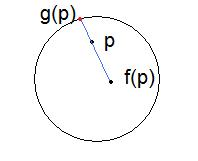
\includegraphics{circlemap}}
\end{figure}

Small variations in $p$ cause small variations in $g(p)$, so this map is continuous. Also note that every point on the circle $S^1$ is sent to itself by $g$, so we say $g$ is a \textbf{retraction}.

Now we claim that such a map cannot exist! The key idea is that the topology of $S^1$ and $D^2$ are different. To make this more precise, we look at loops (closed curves) in $S^1$ and $D^2$. In the disk $D^2$, every loop can be continuously shrunk down to a point, for example by choosing any point and scaling down with respect to this point. On the circle $S^1$, however, this is not true, for example take the path going counterclockwise once.\footnote{This requires a technical argument, which we omit here. We refer the interested reader to~\cite{Hat}, or to the blog post http://holdenlee.wordpress.com/2010/07/02/fundamental-theorem-of-algebra/} 

Consider the path going around the circle once in $D^2$. There exist paths $\gamma_t$ that deform continuously from $t=0$ to $t=1$, such that $\gamma_0$ is the circle and $\gamma_1$ is a point. Taking the images under $f$, we get that the path going once around the circle in $S^1$ can be shrunk down to a point {\it while staying in $S^1$}, which we just said was impossible.

\begin{figure}[h!]
\centering{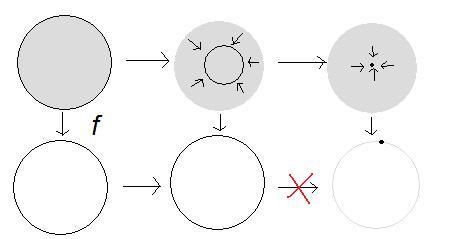
\includegraphics{brouwer}}
\end{figure}

Thus our assumption was wrong, and there must be a fixed point.
\end{proof}
A generalization to $n$ dimensions holds by the same argument, however the intuitive topological fact we need becomes harder to prove.
\begin{exr}
Use topology to prove the Fundamental Theorem of Algebra: Every nonconstant polynomial with constant coefficients has a complex zero. ({\it Hint: follow the steps below.})
\begin{enumerate}
\item 
Suppose that $g$ has no complex zero. Write $g(x)=a_0+\cdots +a_nx^n$, where $a_0\neq 0$. Let $x$ vary around the circle of radius $r$ in the complex plane, i.e. consider $x(t)=re^{2\pi it}=\cos(2\pi t)+i\sin(2\pi t)$ for $0\leq t\leq 1$. What does this look like for small $r$ (particularly $r=0$) versus large $r$? Show that for large $r$, the curve $g(x(t))$ can be continuously deformed {\it without passing through 0} into a circle going $n$ times around the origin.
\item
Under our assumption, the curve $g(x(t))$ varies continuously as $r$ varies, without passing through 0. Why?
\item
Using the fact that a circle going around the origin $n\neq 0$ times cannot be continuously deformed into a point without passing through the origin, conclude that $g$ is constant.
\end{enumerate}
When one curve can be continuously deformed into another, we say that the two curves are {\textbf{homotopic}}.
\end{exr}
We end with a difficult problem where topology comes to the rescue in a surprising way.
\begin{thm}
Any simple closed curve in the plane has an inscribed rectangle.
\end{thm}
\begin{figure}[h!]
\centering{
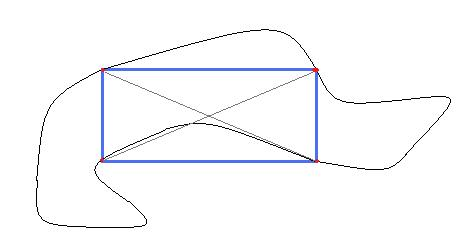
\includegraphics{rectangle}}
\end{figure}
(A simple closed curve is the image of a continuous function $f$ from $[0,1]$ to the plane, with $f(0)=f(1)$, and such that it doesn't intersect itself.)
\begin{proof}
What are characteristic properties of rectangles? We know their opposite sides are parallel, but this requires that we consider each pair of adjacent points. Another characteristic property is that their diagonals are the same length and that they bisect each other. This only requires us to compare two pairs of points. Rephrasing our problem, we want two pairs of distinct points $(A_1,B_1)$ and $(A_2,B_2)$ on our curve $\gamma$ such that the distances $A_1B_1$ and $A_2B_2$ are equal, and such that the midpoints of $\overline{A_1B_1}$ and $\overline{A_2B_2}$ coincide.

We use the idea of {\it geometric continuity}, i.e. when we vary our points by a little bit, that the properties we care about---here, the midpoints of our pair and the distance between them---change by a little bit. To combine our two pieces of information, we think of our plane as embedded in 3-dimensional space, and given two points $A,B$ on  the curve, we define the function $f(A,B)$ as being the point at a distance of $AB$ above the midpoint of $\overline{AB}$. Then $f$ is a map from the {\it space of pairs of points of $\gamma$} into 3-dimensional space. 
Two pairs $(A_1,B_1)$ and $(A_2,B_2)$ have the same distance and midpoint if and only if $f(A_1,B_1)=f(A_2,B_2)$.

\begin{figure}[h!]
\centering{
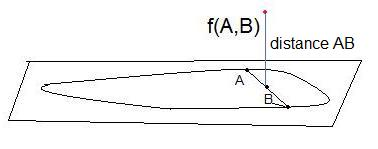
\includegraphics{graph}}
\end{figure}

Suppose by way of contradiction that that $f$ sends different pairs of points to different points. Then $f$ is a one-to-one map from the {\it space of pairs of points of $\gamma$} into 3-dimensional space. What exactly is this ``space"? The curve is parameterized by $[0,1]$ with 0 identified with 1, so specifying an ordered pair of points is like specifying a point in $[0,1]^2$, with the top of the square identified with the bottom and the left identified with the right, i.e. the space of unordered points on the curve can be thought of as the torus. (Glue the sides with the same-colored arrows to see this.)

\begin{figure}[h!]
\centering{
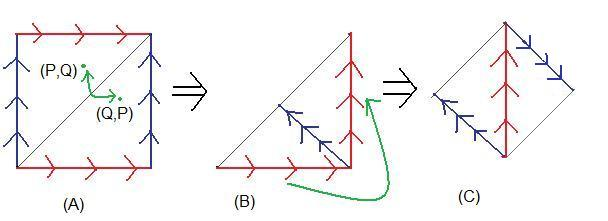
\includegraphics{mobius_diagram}}
\end{figure}

However, we care about {\it unordered} pairs (i.e. sets) of points, so we want to consider $(P,Q)$  and $(Q,P)$ the same. This is like identifying each point in the square with its reflection, so we just consider half the square as in (B). What is the resulting space? This is easier to see if we do a bit of cutting and pasting to get (C); then carrying out the gluing shows that it is a M\"obius strip. Note the diagonal is the set of pairs $(P,P)$, which forms the boundary of the M\"obius strip.

\begin{figure}[h!]
\centering
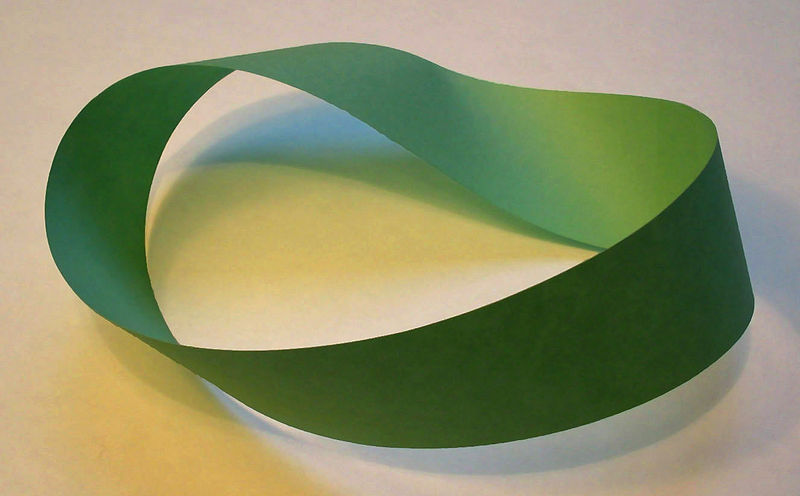
\includegraphics[scale=0.25]{mobius}\\
\caption{
M\"obius strip (from http://en.wikipedia.org/wiki/File:M\%C3\%B6bius\_strip.jpg)}
\end{figure}

Since $f$ is one-to-one, it embeds the M\"obius strip into 3-dimensional space, with the boundary being sent to $\gamma$. But this is impossible---try making a M\"obius strip and gluing its edge onto a curve drawn on a piece of paper! Indeed, it's known from topology that a M\"obius strip with its edges glued together with a ``cap" cannot be embedded into 3-dimensional space. (The proof depends on the fact that the M\"obius strip is not orientable.) Thus $f$ can't be one-to-one; there must be two pairs of points that get sent to the same point, and those pairs of points form the vertices of a rectangle. 
\end{proof}
It is an unsolved problem whether we can always find an inscribed square.
\begin{thebibliography}{9}
\bibitem{CG} Conway, J., and Guy, R.:``The Book of Numbers," Springer-Verlag, NY, 1996.
\bibitem{GKH} Graham, R., Knuth, D., and Patashnik, O.: ``Concrete Mathematics," Addison-Wesley, MA, 1988.
\bibitem{Hat} Hatcher, A.: ``Algebraic Topology," Cambridge University Press, 2002.
%\bibitem{Kra} Krantz, S.:``Techniques of Problem Solving," American Mathematical Society, RI, 1997. OR 
\bibitem{Nie} Nielsen, M.: ``Figures Inscribed in Curves," http://www.webpages.uidaho.edu/$\sim$ markn/squares/.
\end{thebibliography}
\end{document}